\documentclass[10pt,a4paper,parskip=half]{scrartcl}
\usepackage[utf8]{inputenc}
\usepackage{amsmath}
\usepackage{amsfonts}
\usepackage{amssymb}
\usepackage{mathpazo}
\usepackage{tikz}
\usetikzlibrary{patterns}
\usepackage{stmaryrd} % Für den Widerspruchsblitz :D
\usepackage[a4paper,
left=3.0cm, right=3.0cm,
top=2.0cm, bottom=2.0cm]{geometry}
\usepackage{fullpage}
\usepackage[german]{babel}
\usepackage{enumerate}
\setlength{\unitlength}{1cm}
\newcommand{\N}{\mathbb{N}}
\newcommand{\A}{\mathcal{A}}
\newcommand{\R}{\mathbb{R}}
\parindent 0mm
\author{Tom}
\title{Analysis 2 - Hausaufgabe 8}

% new commands for vectors
\newcommand{\vectwo}[2]{\begin{pmatrix}#1\\#2\\\end {pmatrix}}
\newcommand{\vecthree}[3]{\begin{pmatrix}#1\\#2\\#3\\\end {pmatrix}}

\usepackage{listings}
\usepackage{courier}
 \lstset{
         basicstyle=\footnotesize\ttfamily, % Standardschrift
         %numbers=left,               % Ort der Zeilennummern
         numberstyle=\tiny,          % Stil der Zeilennummern
         %stepnumber=2,               % Abstand zwischen den Zeilennummern
         numbersep=5pt,              % Abstand der Nummern zum Text
         tabsize=2,                  % Groesse von Tabs
         extendedchars=true,         %
         breaklines=true,            % Zeilen werden Umgebrochen
         keywordstyle=\color{red},
    		frame=b,         
 %        keywordstyle=[1]\textbf,    % Stil der Keywords
 %        keywordstyle=[2]\textbf,    %
 %        keywordstyle=[3]\textbf,    %
 %        keywordstyle=[4]\textbf,   \sqrt{\sqrt{}} %
         stringstyle=\color{white}\ttfamily, % Farbe der String
         showspaces=false,           % Leerzeichen anzeigen ?
         showtabs=false,             % Tabs anzeigen ?
         xleftmargin=17pt,
         framexleftmargin=17pt,
         framexrightmargin=5pt,
         framexbottommargin=4pt,
         %backgroundcolor=\color{lightgray},
         showstringspaces=false      % Leerzeichen in Strings anzeigen ?        
 }
 \usepackage{caption}
\DeclareCaptionFont{white}{\color{white}}
\DeclareCaptionFormat{listing}{\colorbox[cmyk]{0.43, 0.35, 0.35,0.01}{\parbox{\textwidth}{\hspace{15pt}#1#2#3}}}
\captionsetup[lstlisting]{format=listing,labelfont=white,textfont=white, singlelinecheck=false, margin=0pt, font={bf,footnotesize}}

\usepackage{color}
\usepackage{enumerate}



\begin{document}
\begin{center}
\textsc{\Large{Analysis 2 - Hausaufgabe 8}} \\
\end{center}
\begin{tabbing}
Tom Nick \hspace{1.4cm}\= 342225\\
Tom Lehmann\> 340621\\
Maximilian Bachl\> 341455
\end{tabbing}
\section*{Aufgabe 1}
	\begin{enumerate}[(a)]
\item Wir wissen bereits, dass $\vec{v}$ wirbelfrei ist und ein Potential besitzt (Da $\vec{u}$ ein Potential ist. Da $\vec{v}$ konvex und offen ist, ist eine hinreichende Bedingung damit $\vec{u} + \text{grad} f$ ein Vektorpotential von $\vec{v}$ ist, dass gilt:
\begin{enumerate}[1.]
\item $\text{rot} (\vec{u} + \text{grad} f) = 0 $ \\
\begin{align*}
\text{rot} (\vec{u} + \text{grad} f) &= \text{rot} \vec{u} + \text{rot}(\text{grad} f) \\
&= 0 + \text{rot}(\text{grad} f) \\
&\Leftrightarrow \text{rot}(\text{grad} f) = 0 \\
&=\text{rot}\vecthree{\frac{\partial f}{\partial x}}{\frac{\partial f}{\partial y}}{\frac{\partial f}{\partial z}} \\
&= \begin{pmatrix} \frac{\partial}{\partial y}\frac{\partial f}{\partial z} - \frac{\partial}{\partial z}\frac{\partial f}{\partial y} \\ -\frac{\partial}{\partial x}\frac{\partial f}{\partial z} + \frac{\partial}{\partial z}\frac{\partial f}{\partial x} \\ \frac{\partial}{\partial x}\frac{\partial f}{\partial y} - \frac{\partial}{\partial y}\frac{\partial f}{\partial x}
\end{pmatrix} \\
&= 0
\end{align*}

\end{enumerate}
\item 
\begin{enumerate}[(i)]
	\item 
Da $\vec v$ stetig differenzierbar und $D$ konvex sowie offen ist, muss nur noch geprüft werden ob gilt:
\begin{align*}
\operatorname{div} ( \vec v ) &= 0\\
&= \cos(x) + \frac 23(x+y)^{-\frac 13} - \cos (x) - \frac 23(x+y)^{-\frac 13} = 0\\
\end{align*}
Damit ist gezeigt, dass ein Vektorpotential für $\vec v$ existiert.
\item 
Da $\vec v$ stetig differenzierbar ist und $D$ konvex sowie offen ist, muss nur noch geprüft werden ob gilt:
\begin{align*}
\text{rot} \vec v &= \vec 0\\
&= \begin{pmatrix}
\left(-\cos(x)z-\frac 23(x+y)^{-\frac 13}z \right)\frac {\partial}{\partial y} - (x+y)^{\frac 23} \frac{\partial}{\partial z} \\
\left(z^2  + \sin(x)\right) \frac{\partial}{\partial z} -\left(-\cos(x)z-\frac 23(x+y)^{-\frac 13}z \right) \frac{\partial}{\partial x}\\
(x+y)^{\frac 23} \frac{\partial}{\partial x} - \left( z^2 + \sin(x) \right) \frac{\partial}{\partial y}
\end{pmatrix}\\
&= \begin{pmatrix}
-\frac 29(x+y)^{-\frac 43}z -0 \\
...\\
....\\
\end{pmatrix} \neq \vec 0
\end{align*}
$\vec v$ besitzt somit kein Potential, da die hinreichende Bedingung nicht erfüllt ist.
\end{enumerate}
\end{enumerate}
\subsection*{Aufgabe 3}
\begin{enumerate}[$\quad$]
	\item \ \\ 
	\begin{minipage}{0.50\columnwidth}
	Bei $\vartheta$ konstant entstehen jeweil zwei Kegel die an der z-Achse ausgerichtet sind und jeweils in die andere Richtung gucken. Der gewählte Winkel entscheidet den Winkel der Kegel. Interesassante Spezialfälle sind 0 und $\frac{\pi}{2}$. Bei 0 ist die resultierende Fläche im Grunde nicht vorhanden bzw. ist die z-Achso, bei $\frac{\pi}{2}$ ist eine Fläche entlang der x bzw y Achse.
	\begin{lstlisting}[caption= Mathematica Code für den Graph von f]
	ParametricPlot3D[{r*Sin[2] Cos[z], r*Sin[2] Sin[z], r*Cos[2]}, 
	{z, 0, 2 \[Pi]}, {r, -10, 10}, PlotStyle -> None, 
	BoundaryStyle -> Black]
	\end{lstlisting}
	\end{minipage}
	\begin{minipage}{0.50\columnwidth}
	\begin{center}
	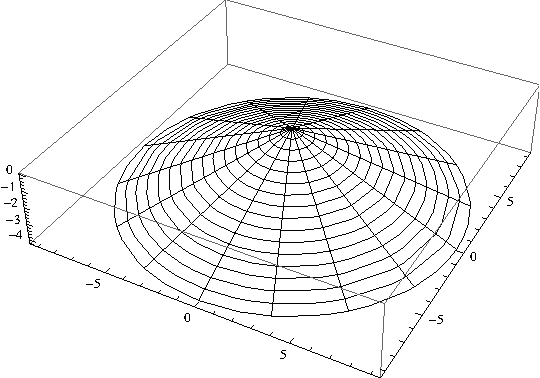
\includegraphics[scale=0.7]{thetakonstant.pdf} 
	\end{center}
	\end{minipage}
	\item \ \\
	\begin{minipage}{0.50\columnwidth}
	Bei $\varphi$ konstant entsteht eine Fläche die auf der z-Achse steht und je nach gewähltem $\varphi$ sich auf der z-Achse dreht.
	\begin{lstlisting}[caption= Mathematica Code für den Graph von f]
	ParametricPlot3D[{r*Sin[y] Cos[0], r*Sin[y] Sin[0], r*Cos[y]}, 
	{y, 0, \[Pi]}, {r, -2, 2}, PlotStyle -> None, 
	 PlotRange -> {{-1, 1}, {-1, 1}, {-1, 1}}]
	\end{lstlisting}
	\end{minipage}
	\begin{minipage}{0.50\columnwidth}
	\begin{center}
	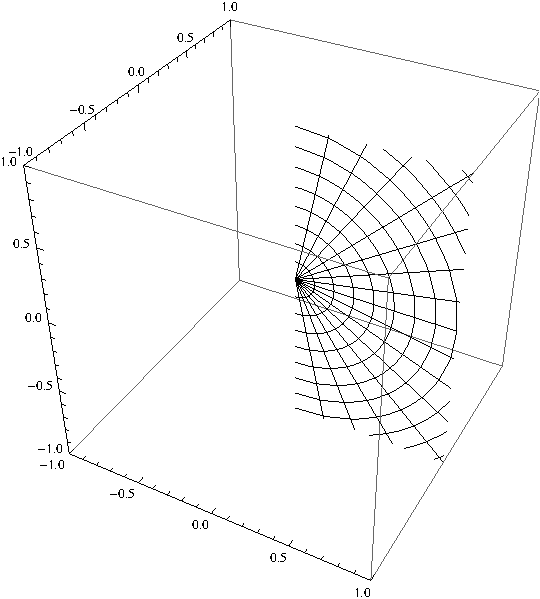
\includegraphics[scale=0.7]{phikonstant.pdf} 
	\end{center}
	\end{minipage}
	\item 	\ \\
	\begin{minipage}{0.50\columnwidth}
	Bei $\varphi$ konstant entsteht eine Fläche die auf der z-Achse steht und je nach gewähltem $\varphi$ sich auf der z-Achse dreht.
	\begin{lstlisting}[caption= Mathematica Code für den Graph von f]
	ParametricPlot3D[{Sin[y] Cos[z], Sin[y] Sin[z], Cos[y]}, 
	{z, 0, 2 \[Pi]}, {y, 0, \[Pi]}, PlotStyle -> None]
	\end{lstlisting}
	\end{minipage}
	\begin{minipage}{0.50\columnwidth}
	\begin{center}
	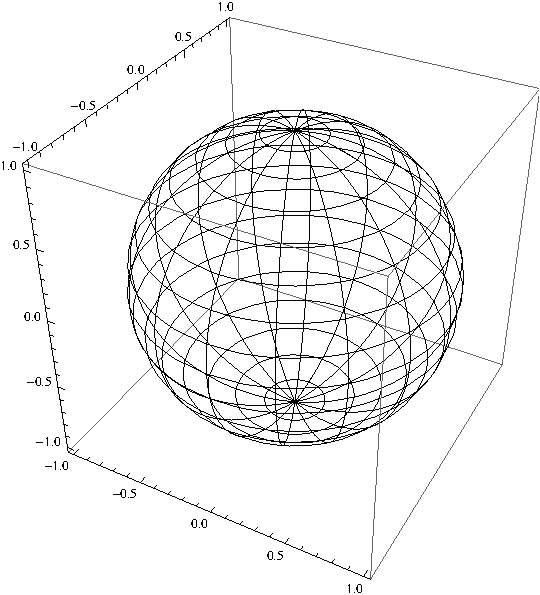
\includegraphics[scale=0.7]{rkonstant.pdf} 
	\end{center}
	\end{minipage}

\end{enumerate}
\end{document}